\section{Survey}
\label{sec:survey}
In order to understand whether the tickets were similar to real tickets, we conducted a survey internal to the company. We were not able to get real data from the company's HR due to the sensitive nature of the data. In order to avoid any ethical implications, we decided to conduct our assessment without involving any real personal data or situations. \todo[inline]{In order to avoid any ethical implications, we decided to conduct our assessment without involving any real personal data or situations.} \\
We asked to some collegues to \todo[inline]{act as the automatic text generator, filling}act as the automatic text generator, filling out a form in an Excel file, where the users were given twenty random prompts, similar to the ones that are given to the GPT model. \\
After giving a brief explanation of the project and what we were trying to achieve, we recommended the users not to use their personal information while writing the fake tickets, but to use the same style of text and the same vocabulary they would use in a real situation. \\
For each ticket, there were several information attached that appeared over all the tickets, which were: name of the person, category of the ticket, sub category of the ticket and some information that were specific to the ticket's category, for example for the category-sub\_category 'Salary - Salary Raise' the additional information given was the new requested salary. \\
We asked the users not to use necessarly all the information that were present in the prompts, but only the ones that felt natural to use, and to slightly change them if it made sense to them ( Ex: Sick leave from Oct 20 2022 can become 'from this Thursday, the 20') \\
Each user was given twenty different prompts sampled randomly from a set of 800 total prompts, belonging to the same categories-sub\_categories of our taxonomy. The prompts contained only the contextual information of the ticket and no ticket's text, so, unlike the prompts used for the GPT models, there were no initial text such as 'Dear Sir/Madame, I would like to \dots' \\
The respondents were also asked to tick the information that they used, and these information were supposed to be used as testing in the NER use case. However, many people either did not tick any information or they ticked only partially what they used, therefore in the end we did not make use of these data. \\\\

\begin{figure}[!h] 
    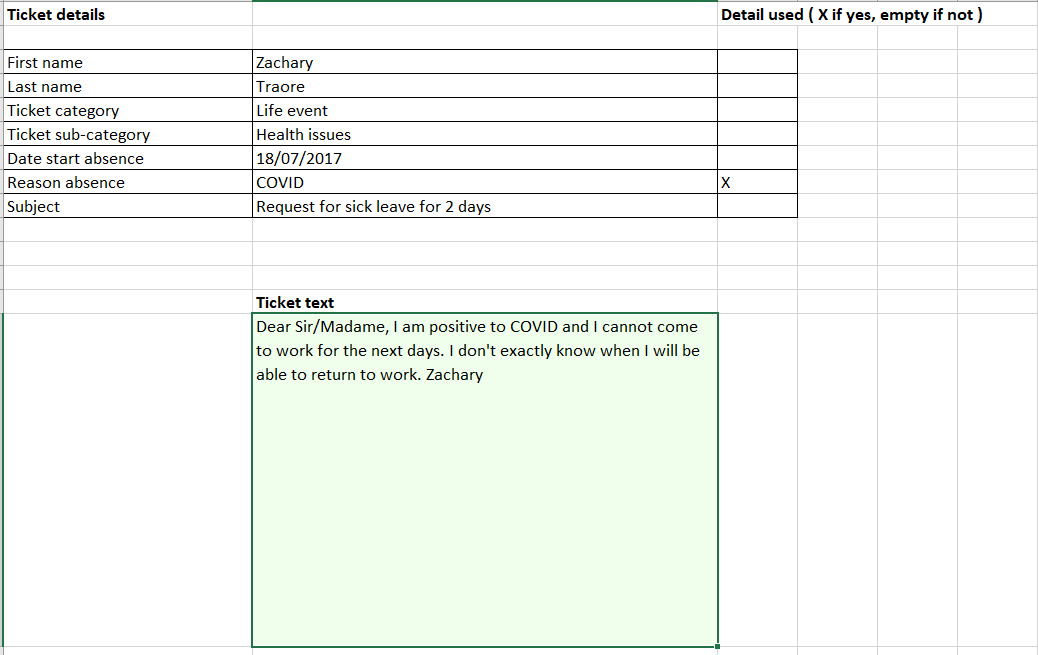
\includegraphics[width=\textwidth]{images/excel_schema_v2.PNG}
    \caption{Example of survey}\todo[inline]{you can explain here what parts are generated, what is the expected user input, and whether this text was produced by a natural person or not}
    \label{fig:survey}
\end{figure}


